\documentclass[12pt,a4paper]{article}

\usepackage{polski}
\usepackage{indentfirst}
\usepackage{graphicx}
\usepackage{fancyhdr}
\usepackage{lastpage}
\usepackage{hyperref}
\usepackage{biblatex}
\usepackage{enumitem}
\usepackage{lmodern}

\title{Specyfikacja implementacyjna projektu grupowego z przedmiotu \textit{Algorytmy~i~struktury~danych}}
\author{Krzysztof Kowalski, Szymon Motłoch, Aleksander Wodnicki}
\date{17 grudnia 2020}

\begin{document}
\maketitle
\thispagestyle{empty}
\newpage
\pagestyle{fancy}
\fancyhf{}
\rhead{Specyfikacja implementacyjna projektu grupowego z przedmiotu \textit{AiSD}}
\rfoot{Strona \thepage \hspace{1pt} z \pageref{LastPage}}
\tableofcontents
\newpage

\section{Wstęp}
\subsection{Cel dokumentu} %OK
Niniejszy dokument przybliża informacje związane z projektem grupowym z przedmiotu \textit{Algorytmy i struktury danych} od strony programistycznej i opisuje strukturę poszczególnych klas i przedstawia zawarte w nich metody. Znajdują się tu również informacje dotyczące sposobu wersjonowania kodu źródłowego, a także informacje o testach jednostkowych oraz wykorzystany algorytm.

Użytkownik, po zapoznaniu się z tym dokumentem, powinien być w stanie napisać na jego podstawie działający program, który zrealizuje założenia projektowe.

\subsection{Cel projektu} %OK
Celem projektu, jak to zostało opisane również w specyfikacji funkcjonalnej, jest stworzenie programu, który pomoże rozwiązać problem opisany w~dziale o tej samej nazwie, we wspomnianej specyfikacji funkcjonalnej. Program, po uruchomieniu i otrzymaniu pliku z danymi o szpitalach, drogach między nimi oraz o obiektach na mapie, analizuje go i wyświetla mapę na graficznym interfejsie. Program otrzymuje również plik z danymi o miejscu pobytu pasażerów lub też otrzymuje te dane z poziomu interfejsu graficznego, po podaniu ich przez użytkownika w przeznaczonych do tego opisanych polach. Znając te informacje, program będzie pokazywać trasę karetki pogotowia od momentu odbioru pacjenta, przez przejście kolejnych, najbliższych szpitali, aż do momentu znalezienia się szpitala, w którym są wolne łóżka lub dotarcia do ostatniego nieodwiedzonego szpitala. 

\subsection{Środowisko pracy} %OK
Praca nad programem będzie odbywała się na 64-bitowym systemie \textit{Windows 10 Home} (wersja \textit{2004}, build \textit{19041.685}) w programie \textit{Apache NetBeans IDE} (wersja \textit{11.3 LTS}) w \textit{JDK 8}.
\newpage

\subsubsection{Parametry stacji roboczej} %TBC
Poniżej opisane zostały podzespoły urządzeń, na których opracowany jest projekt:
\begin{enumerate}
\item Laptop 1:
\begin{itemize}
\item model: HP Pavilion Gaming 15-cx0006nw
\item procesor: Intel Core i5-8300H (2.3 GHz, 4.0 GHz Turbo, 8 MB Cache)
\item pamięć RAM: DDR4 (2666 MHz) 8 GB
\item dyski twarde: SSD 240 GB; HDD 1000 GB
\item karta graficzna: Nvidia Geforce GTX 1050 4 GB
\item system operacyjny: Microsoft Windows 10 Home.
\end{itemize}
\item Laptop 2:
\begin{itemize}
\item model: Latitude E5250
\item procesor: Intel Core i5-5300U CPU @ 2.30GHz  2.29GHz
\item pamięć RAM: 8 GB
\item dyski twarde: Samsung SSD 850 EVO 1TB 
\item karta graficzna: Intel(R) HD Graphics 5500
\item system operacyjny: Microsoft Windows 10 Pro.
\end{itemize}
\item Laptop 3:
\begin{itemize}
\item model: Acer Aspire 7 
\item procesor: Intel Core i5-7300U CPU @ 2.50GHz  3.5GHz
\item pamięć RAM: 16 GB
\item dyski twarde: SSD 500 GB; HDD 1000 GB
\item karta graficzna: Nvidia Geforce GTX 1050 2 GB
\item system operacyjny: Microsoft Windows 10 Home.
\end{itemize}
\end{enumerate}

\subsubsection{Kompilator i język programowania} %OK
Jak opisano wcześniej, językiem programowania używanym przy tym projekcie, będzie język \textit{Java}. Kompilacja odbędzie się dzięki programowi \textit{javac}, a uruchamianie za pomocą programu \textit{java}. Alternatywą dla tego rozwiązania jest skorzystanie ze środowiska programistycznego (np. \texttt{NetBeans}) w celu kompilacji oraz uruchomienia programu.

\section{Sposób wersjonowania} %OK
Wszystkie zmiany w kodzie źródłowym będą rejestrowane w zdalnym repozytorium, które znajduje się po wejściu w poniższy link:\begin{center}
\small{\texttt{https://projektor.ee.pw.edu.pl/repo/git/2020Z\_AISD\_proj\_zesp\_GR3\_gr10}}
\end{center}
Wersjonowanie zaś będzie realizowane zgodnie z poniższym schematem:
\begin{center}
\texttt{X.Y.Z}
\end{center}
\texttt{X} oznacza etap rozwoju programu (0 – faza początkowa, pojedyncze metody, 1 – podstawowa funkcjonalność etc.), \texttt{Y} to kolejne znaczne poprawki wprowadzone do kodu źródłowego, a \texttt{Z} to ewentualne drobne poprawki (np.~literówki, usunięcie komentarzy, zmiana nazwy zmiennej).
Zmiany w kodzie będą dokonywane na gałęzi \texttt{master} - każdy \textit{push}, oprócz kolejnej wersji kodu, dostarczy również komentarz i tag z wersją tego kodu. Zostanie również utworzony plik w~formacie \texttt{.txt}, w którym to zostaną opisane zmiany wprowadzone w danej wersji.


\section{Algorytm} %TBC

Algorytmem, który zostanie wykorzystany przy realizacji omawianego projektu będzie przykład algorytmu zachłannego – \texttt{algorytm Dijkstry}.

Algorytm ten rozwiązuje jeden z klasycznym problemów w teorii grafów związany ze znajdowaniem ścieżki między dwoma wierzchołkami, w tym przypadku ścieżki najkrótszej. Działa on wtedy, gdy mamy do czynienia z~krawędziami o wartościach nieujemnych, tak że w przypadku tego problemu będzie on najbardziej odpowiedni, gdyż odległość między szpitalami nie może być ujemna.

Algorytm Dijkstry znajduje w grafie wszystkie ścieżki od wierzchołka początkowego do docelowego oraz wylicza koszt ich przejścia, czyli w naszym przypadku przejechaną przez karetkę odległość. W ten sposób pomaga on wyznaczyć ścieżkę najkrótszą, która jest niezbędna do realizacji założeń projektowych.

Złożoność tego algorytmu jest zależna od wykorzystanych struktur oraz od liczby \texttt{$V$} wierzchołków i krawędzi \texttt{$E$} w danym grafie. W~przypadku skorzystania ze zwykłych tablic, złożoność określimy jako \texttt{$O(V^{2})$}, zaś w przypadku kopca, ten sam algorytm będzie określony za pomocą złożoności \texttt{$O(ElogV)$}. Pierwsza z nich jest najbardziej optymalna w przypadku grafów gęstych, gdzie liczba krawędzi jest większa od liczby wierzchołków, druga najbardziej optymalna w przypadku przeciwnym, kiedy to liczba wierzchołków jest większa od krawędzi tego grafu.
\newpage

\section{Diagram klas}

Poniżej został przedstawiony diagram klas programu:

\begin{figure}[h!]
\centering
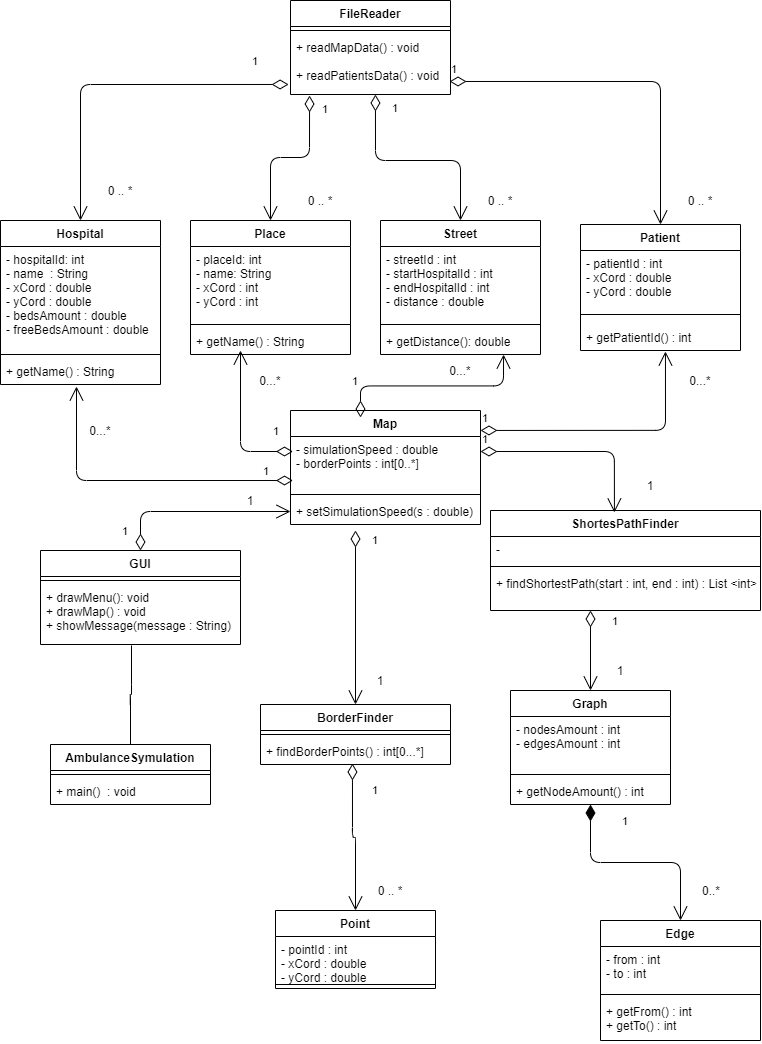
\includegraphics[width=0.95\textwidth]{Diagram}
\caption{Diagram klas} 
\label{fig:Diagram}
\end{figure}

\subsection{Opis klas}
Poniżej przestawiono listę klas z powyższego diagramu, dodatkowo zamieszczono krótki opis każdej z nich:
\begin{itemize}
\item \textbf{AmbulanceSymulation} - klasa zawierająca metodę \texttt{main}, która uruchamia wszystkie elementy programu;
\item \textbf{FileReader} - klasa służąca do wczytywania danych wejściowych z pliku;
\item \textbf{Hospital} – klasa reprezentują dane szpitali;
\item \textbf{Place} – klasa reprezentująca dane obiektów;
\item \textbf{Street} – klasa reprezentująca dane dróg łączących szpitale;
\item \textbf{Patient} – klasa reprezentująca dane pacjentów;
\item \textbf{Graph} – klasa reprezentująca grafy;
\item \textbf{Edge} – klasa reprezentująca krawędzie grafu;
\item \textbf{ShortesPathFinder} – klasa umożliwiająca wyznaczanie najkrótszej ścieżki między dwoma punktami na postawie dostarczonego spisu wszystkich dróg;
\item \textbf{BorderFinder} – klasa umożliwiająca znalezienie granic państwa na bazie istniejących szpitali i obiektów;
\item \textbf{Map} – klasa przechowująca wszystkie dane związane ze stanem mapy;
\item \textbf{GUI} – klasa generująca interfejs użytkownika;
\item \textbf{Point} – klasa reprezentująca punkt na mapie ze współrzędnymi X i Y.
\end{itemize}

\section{Testowanie}
Jak przedstawiono w specyfikacji funkcjonalnej dla tego projektu, testowanie będzie odbywało się z wykorzystaniem testów jednostkowych \textit{JUnit~5}, dodatkowo również napisane zostaną testy jednostkowe, w których skorzystamy z \textit{AssertJ} – te będą stanowiły większą część testów. Wszystkie testy zostaną przygotowane tak, aby przetestować możliwie jak najwięcej metod, ale także plików w formacie \texttt{.txt}, w celu sprawdzenia reakcji programu na nie. Testy jednostkowe zostaną umieszczone w klasach testowych odpowiednich dla testowanych metod (np. metoda \textit{x} pochodzi z klasy \textit{y}, więc klasa testowa będzie nosiła nazwę \textit{yTest}).

\begin{thebibliography}{1}
\bibitem{Opis Problemu}
ISOD — Wirtualny Dziekanat:
\texttt{isod.ee.pw.edu.pl}
\end{thebibliography}

\end{document}